\documentclass[11pt,a4paper]{article}

\usepackage[margin=2.5cm]{geometry}
\usepackage{amsmath,amssymb,amsthm}
\usepackage{booktabs}
\usepackage{microtype}
\usepackage{enumitem}
\usepackage[dvipsnames]{xcolor}
\usepackage{tikz}
\usepackage[most]{tcolorbox}
\usepackage[hidelinks]{hyperref}

\newtheorem{definition}{Definition}[section]
\newtheorem{lemma}[definition]{Lemma}
\newtheorem{proposition}[definition]{Proposition}
\theoremstyle{remark}
\newtheorem{remark}[definition]{Remark}

% Plain-language boxes open every section; example boxes carry worked numbers.
\newtcolorbox{plain}{enhanced,colback=Blue!4,colframe=Blue!45,boxrule=0.6pt,arc=2pt,
  left=6pt,right=6pt,top=4pt,bottom=4pt,
  title={In plain words},fonttitle=\bfseries\small,coltitle=Blue!70!black,
  colbacktitle=Blue!10,attach boxed title to top left={xshift=6pt,yshift=-2pt},
  boxed title style={boxrule=0pt,arc=1pt}}
\newtcolorbox{example}[1]{enhanced,colback=Gray!5,colframe=Gray!55,boxrule=0.6pt,arc=2pt,
  left=6pt,right=6pt,top=4pt,bottom=4pt,
  title={Example: #1},fonttitle=\bfseries\small,coltitle=black,
  colbacktitle=Gray!15,attach boxed title to top left={xshift=6pt,yshift=-2pt},
  boxed title style={boxrule=0pt,arc=1pt}}

\newcommand{\cells}{\mathcal{C}}
\newcommand{\types}{\mathcal{T}}
\newcommand{\lab}{\ell}
\newcommand{\obs}{\mathrm{obs}}
\newcommand{\Nb}[1]{N_{#1}}
\newcommand{\ind}[1]{\mathbf{1}\!\left[#1\right]}
\newcommand{\Real}{\mathbb{R}}
\newcommand{\Nat}{\mathbb{Z}_{\ge 0}}

\title{PaM-ST: what the pipeline does, and why it can be trusted}
\author{}
\date{18 September 2026}

\begin{document}
\maketitle

\begin{abstract}
This note explains what \texttt{pam\_st} computes when run with
\texttt{--statistic minp}, the significance search that reports the motifs
least explained by chance, for one tissue or for several analysed together.
Every idea is given three times: in plain words, as mathematics, and as a small
worked example with exact numbers. The plain-language boxes can be read on
their own; the definitions and propositions state precisely what the code
implements and under which assumptions its $p$-values are valid.
Section~\ref{sec:evidence} reports the simulations that check those
guarantees, and Section~\ref{sec:real} a run on four PDAC tissues.
\end{abstract}

\tableofcontents

% =====================================================================
\section{The picture: cells, circles and recipes}
\label{sec:data}

\begin{plain}
Think of a tissue as a huge map covered in marbles glued in place. Each marble
is a cell and its colour is the cell type. Around every marble we draw a small
circle and write down what is inside: say \emph{5 red and 3 blue}. That list is
a \emph{recipe}. We care about the mix, not the size: \emph{5 red, 3 blue} and
\emph{10 red, 6 blue} are the same recipe. Two recipes count as matching when
their mixes are almost the same. A \emph{motif} is a recipe that keeps coming
back.
\end{plain}

\begin{definition}[Tissue]
A tissue is a finite set of cells $\cells=\{1,\dots,n\}$ with positions
$x_i\in\Real^2$ and labels $\lab_i\in\types=\{1,\dots,K\}$; the labelling is
$\lab=(\lab_1,\dots,\lab_n)$. Cells annotated \texttt{unclassified} are removed
before analysis. Positions never change; every null model acts on $\lab$ alone.
\end{definition}

\begin{definition}[Neighbourhood and composition]
For a radius $r>0$, $\Nb{i}=\{j\in\cells:\lVert x_j-x_i\rVert_2\le r\}$, which
contains $i$. Its composition under $\lab$ is the count vector $h_i(\lab)\in\Nat^K$,
$h_i(\lab)[t]=|\{j\in \Nb{i}:\lab_j=t\}|$.
\end{definition}

\begin{definition}[Matching]
With \texttt{--metric l2}, write $u(h)=h/\lVert h\rVert_2$ and
$d(h,h')=\lVert u(h)-u(h')\rVert_2\in[0,\sqrt2]$, the chord distance between
directions. With \texttt{--metric js},
\[
  d(h,h')=\sqrt{\operatorname{JS}\bigl(p(h),p(h')\bigr)},\qquad p(h)=h/\mathbf 1^\top h,
\]
the square root of the Jensen--Shannon divergence between proportions. Two compositions \emph{match} when
$d\le\rho$; for $\rho=0$ this is exact proportional equality.
\end{definition}

\begin{definition}[Frequency and disjoint support]
\label{def:freq}
For a query vector $v$ and a set of centres $S$, the \emph{frequency} is
$N(v;\lab,S)=|\{i\in S:d(h_i(\lab),v)\le\rho\}|$. The \emph{disjoint support}
$D(v;\lab,S)$ is the size of the set built by taking matching centres in index
order and keeping each one whose neighbourhood shares no cell with those
already kept.
\end{definition}

Frequency counts overlapping circles separately, so one dense clump counts many
times; disjoint support counts it once. The implementation groups identical
compositions (equal up to a common divisor) into classes and answers one ball
query per class with a KD-tree ($\ell_2$) or a vantage-point tree (JS), which
gives the same $N$.

\begin{example}{how close is ``almost the same''?}
With two types (red, blue) and \texttt{--rho 0.05}:
\begin{center}
\begin{tabular}{lll}
\toprule
Recipe & Compared with $(5,3)$ & Match? \\
\midrule
$(10,6)$ & $d=0$ (same mix, twice the size) & yes \\
$(6,3)$ & $d=0.077$ & no \\
$(5,4)$ & $d=0.134$ & no \\
$(4,4)$ & $d=0.244$ & no \\
\bottomrule
\end{tabular}
\end{center}
A tolerance of $\rho=0.05$ is an angle of $2.87^\circ$ between directions: a
tight match. It also explains an old artefact. The recipe \emph{20
fibroblasts, 1 immune cell} sits at distance $0.04995$ from \emph{pure
fibroblasts}, just inside the tolerance, so it matches every pure-fibroblast
neighbourhood --- which is why the original frequency test kept
reporting \texttt{Other\_fibroblasts:20; Other\_immune:1}.
\end{example}

% =====================================================================
\section{The luck machine: null models}
\label{sec:null}

\begin{plain}
Some recipes come back again and again. Is that because cells really like to
sit that way, or just luck? To find out we build pretend maps: every marble
stays where it is, but we peel off the colour stickers and stick them back on
at random. There is one rule. Some parts of a tissue naturally have more of
one colour, like a forest has more trees than a beach. So we cut the map into
squares and only swap stickers \emph{inside} each square. Every square keeps
exactly its own number of each colour; only the fine arrangement gets mixed
up.
\end{plain}

\begin{definition}[Block null]
Fix a tile side $L>0$ and origin $o$. The tile of $x$ is
$\gamma_L(x)=(\lfloor (x_1-o_1)/L\rfloor,\lfloor (x_2-o_2)/L\rfloor)$, inducing a
partition $\mathcal B=\{B_1,\dots,B_G\}$ of $\cells$. Under $H_0^{\mathrm{blk}}$,
conditional on positions and on the label multiset of every tile, $\lab$ is
uniform over $\Pi_{\mathcal B}=\prod_g\mathfrak S(B_g)$ acting on labels. The
global null is the special case $G=1$.
\end{definition}

\begin{remark}[The draws are independent]
The code applies a fresh uniform within-tile permutation to the previous draw
rather than to $\lab^{\obs}$. A uniform element of $\Pi_{\mathcal B}$ composed
with any fixed arrangement is again uniform and independent of it, so the draws
$\lab^{(1)},\dots,\lab^{(B)}$ are i.i.d.\ from the null.
\end{remark}

\begin{example}{a tissue of eight cells}
\begin{center}
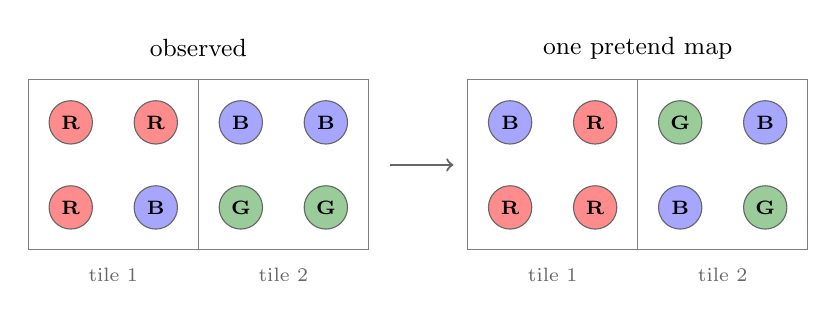
\begin{tikzpicture}[x=0.9cm,y=0.9cm,
    cell/.style={circle,draw=black!60,minimum size=0.55cm,inner sep=0pt,font=\scriptsize\bfseries}]
  \foreach \ox/\title in {0/observed, 6.2/one pretend map} {
    \draw[black!50] (\ox,0) rectangle ++(2.4,2.4);
    \draw[black!50] (\ox+2.4,0) rectangle ++(2.4,2.4);
    \node[font=\small] at (\ox+2.4,2.85) {\title};
    \node[font=\scriptsize,black!60] at (\ox+1.2,-0.35) {tile 1};
    \node[font=\scriptsize,black!60] at (\ox+3.6,-0.35) {tile 2};
  }
  % observed
  \node[cell,fill=Red!45] at (0.6,1.8) {R};   \node[cell,fill=Red!45] at (1.8,1.8) {R};
  \node[cell,fill=Red!45] at (0.6,0.6) {R};   \node[cell,fill=Blue!35] at (1.8,0.6) {B};
  \node[cell,fill=Blue!35] at (3.0,1.8) {B};  \node[cell,fill=Blue!35] at (4.2,1.8) {B};
  \node[cell,fill=Green!40] at (3.0,0.6) {G}; \node[cell,fill=Green!40] at (4.2,0.6) {G};
  % shuffled within tiles
  \node[cell,fill=Blue!35] at (6.8,1.8) {B};  \node[cell,fill=Red!45] at (8.0,1.8) {R};
  \node[cell,fill=Red!45] at (6.8,0.6) {R};   \node[cell,fill=Red!45] at (8.0,0.6) {R};
  \node[cell,fill=Green!40] at (9.2,1.8) {G}; \node[cell,fill=Blue!35] at (10.4,1.8) {B};
  \node[cell,fill=Blue!35] at (9.2,0.6) {B};  \node[cell,fill=Green!40] at (10.4,0.6) {G};
  \draw[->,thick,black!60] (5.1,1.2) -- (6.0,1.2);
\end{tikzpicture}
\end{center}
Tile 1 holds three red and one blue; tile 2 two blue and two green. The block
null allows $\binom41\binom42=4\times6=24$ labellings, each equally likely, and
every one keeps three red and one blue in tile 1. The global null would allow
$8!/(3!\,3!\,2!)=560$ labellings, including ones that move every red cell into
tile 2. The block null is the stricter comparison: it forgives the tissue for
having regions and asks only about the arrangement inside them.
\end{example}

% =====================================================================
\section{How surprising? The \texorpdfstring{$p$}{p}-value}
\label{sec:p}

\begin{plain}
We make many pretend maps --- thousands --- and count the recipe on each. Then
we ask: out of all those maps, how many had the recipe at least as often as the
real one? If hardly any did, luck is a poor explanation. The key idea: if
nothing special were going on, the real map would just be one more pretend map,
equally likely to land anywhere in the line-up. Landing at the very top by
chance happens only one time in $B+1$.
\end{plain}

\begin{definition}[Pooled-rank $p$-value]
\label{def:p}
For a fixed query vector $v$, let $N^{\obs}=N(v;\lab^{\obs},S)$ and
$N^{(b)}=N(v;\lab^{(b)},S)$ for $b=1,\dots,B$. Pool the $B+1$ values into
$\mathcal P=\{N^{\obs},N^{(1)},\dots,N^{(B)}\}$ and let
$R(y)=|\{z\in\mathcal P:z\ge y\}|$. Then
\[
  p=\frac{R(N^{\obs})}{B+1}=\frac{1+|\{b:N^{(b)}\ge N^{\obs}\}|}{B+1},
  \qquad
  p^{(b)}=\frac{R(N^{(b)})}{B+1}.
\]
\end{definition}

\begin{proposition}[Validity]
\label{prop:valid}
If $N^{\obs},N^{(1)},\dots,N^{(B)}$ are exchangeable, then
$\Pr(p\le\alpha)\le\alpha$ for every $\alpha\in(0,1)$, with equality at
multiples of $1/(B+1)$ when ties have probability zero.
\end{proposition}

\begin{proof}
Exchangeability makes the rank of $N^{\obs}$ among the $B+1$ values uniform
(ties only make $R$ larger), so $\Pr(R(N^{\obs})\le k)\le k/(B+1)$.
\end{proof}

\begin{example}{nine pretend maps}
A recipe appears 12 times on the real map. On nine pretend maps it appears
$4,6,3,5,7,2,4,6,5$ times. None reaches 12, so $R(12)=1$ and
$p=1/10=0.1$. That is the smallest $p$ nine maps can ever give: to show that
something happens less than once in a thousand by chance you need thousands of
pretend maps (Section~\ref{sec:budget}).
\end{example}

% =====================================================================
\section{Trap 1: drawing the target after shooting the arrow}
\label{sec:split}

\begin{plain}
If you pick a recipe \emph{because} you saw it a lot, it will of course look
common --- like shooting an arrow and then drawing the target around it. To
avoid this we colour the map like a chessboard. The black squares are used to
\emph{choose} which recipes to test, and the white squares only to
\emph{check} them. A circle is used only if it fits entirely inside its own
square, so a checking circle can never share a marble with a choosing one. And
the pretend maps only shuffle stickers on the white squares: the black squares
stay exactly as they were when the recipes were chosen.
\end{plain}

\begin{center}
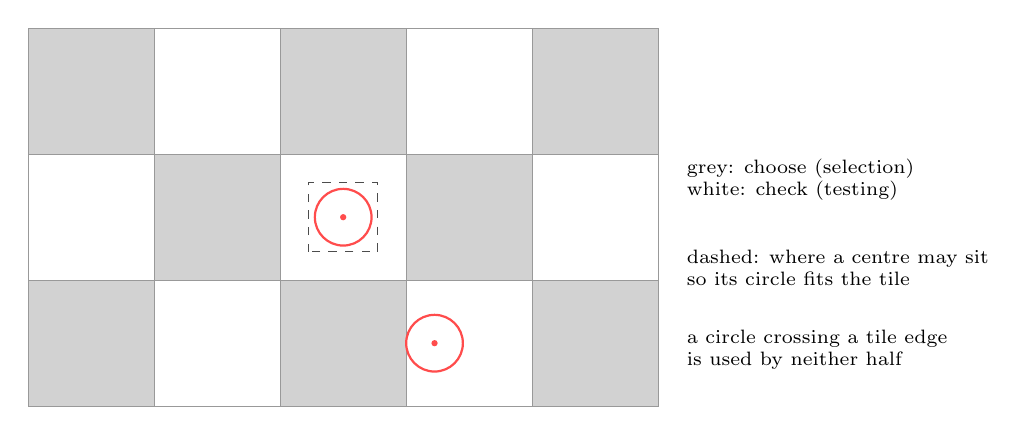
\begin{tikzpicture}[x=0.8cm,y=0.8cm]
  \foreach \i in {0,...,4} \foreach \j in {0,...,2} {
    \pgfmathtruncatemacro{\parity}{mod(\i+\j,2)}
    \ifnum\parity=0 \fill[Gray!35] (\i*2,\j*2) rectangle ++(2,2); \fi
    \draw[black!40] (\i*2,\j*2) rectangle ++(2,2);
  }
  \draw[dashed,black!70] (4.45,2.45) rectangle (5.55,3.55);
  \draw[Red!70,thick] (5.0,3.0) circle (0.45);
  \fill[Red!70] (5.0,3.0) circle (0.05);
  \draw[Red!70,thick] (6.45,1.0) circle (0.45);
  \fill[Red!70] (6.45,1.0) circle (0.05);
  \node[font=\scriptsize,align=left,anchor=west] at (10.3,3.6) {grey: choose (selection)\\white: check (testing)};
  \node[font=\scriptsize,align=left,anchor=west] at (10.3,2.2) {dashed: where a centre may sit\\so its circle fits the tile};
  \node[font=\scriptsize,align=left,anchor=west] at (10.3,0.9) {a circle crossing a tile edge\\is used by neither half};
\end{tikzpicture}
\end{center}

\begin{definition}[Checkerboard split]
Fix a split side $L_s>2r$. For cell $i$ let $\gamma_{L_s}(x_i)=(a,b)$ with lower
corner $c(i)$. Cell $i$ is \emph{interior} when
$\min_k\min(x_{ik}-c_k(i),\,c_k(i)+L_s-x_{ik})\ge r$, and its parity is
$\pi(i)=(a+b)\bmod 2$. Selection centres are $S_0=\{i\text{ interior}:\pi(i)=0\}$,
testing centres $S_1=\{i\text{ interior}:\pi(i)=1\}$. Write $A_0$, $A_1$ for the
cells lying in even and odd split tiles.
\end{definition}

\begin{lemma}[Separation]
\label{lem:sep}
For $i\in S_1$, $\Nb{i}\subseteq A_1$; for $j\in S_0$, $\Nb{j}\subseteq A_0$; hence
$\Nb{i}\cap\Nb{j}=\emptyset$.
\end{lemma}

\begin{proof}
Interiority puts every point within $r$ of $x_i$ inside the closure of $x_i$'s
tile. The test uses non-strict inequalities, so containment can fail only for
a neighbour lying exactly on the upper tile boundary at distance exactly $r$, a
null event for measured coordinates. Tiles of different parity are disjoint.
\end{proof}

\begin{definition}[Candidate family]
\label{def:family}
With support floor $s$ and optional composition filter $(m,c)$,
\begin{align*}
  \mathcal F=\bigl\{\hat h_q:\ &q\text{ a class on }S_0,\
  N(\hat h_q;\lab^{\obs},S_0)\ge s,\ D(\hat h_q;\lab^{\obs},S_0)\ge s,\\
  &|\{t:\hat h_q[t]\ge c\}|\ge m\bigr\}=\{v_1,\dots,v_C\},
\end{align*}
with $\hat h_q$ the first count vector of class $q$; the filter is off when $m=0$.
\end{definition}

\begin{lemma}[Measurability]
\label{lem:meas}
$\mathcal F$ is a function of $\lab|_{A_0}$ alone.
\end{lemma}

\begin{proof}
$\mathcal F$ uses only $h_i(\lab)$ and match sets for $i\in S_0$, whose
neighbourhoods lie in $A_0$ by Lemma~\ref{lem:sep}.
\end{proof}

\begin{definition}[Conditional null]
$H_0^{\mathrm{blk},1}$: conditional on positions, per-tile label multisets and
$\lab|_{A_0}$, the labelling is uniform over $\prod_g\mathfrak S(B_g\cap A_1)$ ---
labels move only within the testing part of each tile.
\end{definition}

\begin{example}{what happened before the split existed}
The first version chose the family and tested it on the same neighbourhoods.
On tissues with uniformly placed cells and independently drawn labels ---
where by construction there is nothing to find --- every dataset that produced
a candidate declared it significant: 5 out of 5. The reason: a recipe that
reached support 10 by chance was chosen \emph{because} it did, while its
pretend-map counts, which never chose it, sat near zero. After the split, none
of 40 such datasets reported anything.
\end{example}

% =====================================================================
\section{Trap 2: buying hundreds of lottery tickets}
\label{sec:wy}

\begin{plain}
We do not test one recipe but hundreds. If you buy 823 lottery tickets, one of
them probably wins by luck. So we ask a tougher question. On every pretend map
we look at the \emph{luckiest} of all the recipes, and a real recipe only
counts if it beats the best that luck could offer anywhere in the list. Then we
repeat without the winner, to judge the second best against the luckiest of
the rest, and so on.
\end{plain}

For the family $v_1,\dots,v_C$, compute $p_c$ and $p^{(b)}_c$ as in
Definition~\ref{def:p}, on the testing centres $S_1$.

\begin{definition}[Westfall--Young step-down on the minimum $p$-value]
Order the candidates so that $p_{(1)}\le\dots\le p_{(C)}$ (ties by decreasing
lift, then first appearance). For $k=1,\dots,C$,
\[
  M^{(b)}_k=\min_{j\ge k}p^{(b)}_{(j)},\qquad
  \tilde p_{(k)}=\frac{1+|\{b:M^{(b)}_k\le p_{(k)}\}|}{B+1},\qquad
  \bar p_{(k)}=\max_{j\le k}\tilde p_{(j)}.
\]
Candidate $c$ is significant when $\bar p_c\le\alpha$.
\end{definition}

\begin{proposition}[Family-wise error]
\label{prop:fwer}
Under $H_0^{\mathrm{blk},1}$ and subset pivotality --- the joint law of the true
nulls' $p$-values does not depend on which other hypotheses are true ---
$\Pr(\exists\ \text{true null } c:\bar p_c\le\alpha)\le\alpha$.
\end{proposition}

This is the Westfall--Young result: the permutations supply the joint law of
the $p$-values, dependence included, so no independence is assumed.

\begin{remark}[Why observation and draws share one pooled set]
Scoring each draw only against the other draws gives it denominator $B$ and a
floor of $1/B$, while the observation reaches $1/(B+1)$. An observation at its
floor could then never be matched, and the adjustment rejected $10$--$16\%$ of
the time at $\alpha=0.05$ on exchangeable counts. Scoring everything inside
the same $B+1$ values restores the nominal level.
\end{remark}

\begin{example}{how many lottery tickets win by luck?}
With 823 candidates that are all pure luck and a $5\%$ threshold each, you
expect $823\times0.05\approx41$ false hits, and the chance of at least one is
$1-0.95^{823}$, indistinguishable from $1$. Without the adjustment, a search
this size \emph{always} finds something.
\end{example}

\begin{example}{three recipes, nine pretend maps}
\small
\begin{center}
\begin{tabular}{lccccccccccc}
\toprule
& real & \multicolumn{9}{c}{pretend maps $b=1,\dots,9$} & raw $p$ \\
\midrule
count of A & 12 & 4 & 6 & 3 & 5 & 7 & 2 & 4 & 6 & 5 & 0.1 \\
count of B &  9 & 5 & 9 & 4 & 10 & 6 & 5 & 3 & 7 & 4 & 0.3 \\
count of C &  3 & 2 & 4 & 3 & 5 & 1 & 3 & 2 & 4 & 3 & 0.7 \\
\midrule
\multicolumn{12}{l}{each pretend map's own pooled rank (numerator of its $p^{(b)}$ over 10)} \\
A & & 8 & 4 & 9 & 6 & 2 & 10 & 8 & 4 & 6 & \\
B & & 7 & 3 & 9 & \textbf{1} & 5 & 7 & 10 & 4 & 9 & \\
C & & 9 & 3 & 7 & \textbf{1} & 10 & 7 & 9 & 3 & 7 & \\
\midrule
luckiest of A, B, C & & 7 & 3 & 7 & \textbf{1} & 2 & 7 & 8 & 3 & 6 & \\
\bottomrule
\end{tabular}
\end{center}
\normalsize
A is the most extreme on the real map (rank 1, raw $p=0.1$). On map $b=4$ the
luckiest recipe --- B, and C too --- also reached rank 1. So A beats
everything luck produced except once: $\tilde p_A=(1+1)/10=0.2$. B is then
judged only against the luckiest of B and C: three maps reach rank $\le3$, so
$\tilde p_B=0.4$. C against itself gives $0.7$. Raw $0.1,0.3,0.7$ become adjusted
$0.2,0.4,0.7$: A pays for the fact that we also looked at B and C.
\end{example}

% =====================================================================
\section{How many pretend maps are enough?}
\label{sec:budget}

\begin{plain}
With 9 pretend maps the best you can ever say is ``one time in ten''. With a
big list of recipes it gets worse: on almost every pretend map \emph{some}
recipe will look as extreme as it can, so the luckiest-of-all bar is almost
always at the top. You then need so many pretend maps that even the luckiest
recipe rarely hits the top. As a rule of thumb, about twenty pretend maps for
every recipe on the list.
\end{plain}

Every $p$-value is a multiple of $1/(B+1)$. If the $C$ candidates behaved
independently, a fraction $\approx C/(B+1)$ of the draws would have some
candidate at its floor, so
\[
  \min_c\bar p_c\ \gtrsim\ \frac{C}{B+1},
  \qquad\text{hence rejecting at level }\alpha\text{ needs }\ B\gtrsim\frac{C}{\alpha}.
\]
Correlated candidates, which near-duplicate recipes are, do better. The
implementation warns when $B+1<20\,C$.

\begin{example}{823 candidates on LSP31891}
With $B=199$ the bound is $823/200\approx4$: no recipe could ever be declared
significant. With $B=19{,}999$ it is $0.041$, and the run reported
significant motifs at $\bar p=0.0136$, below the bound because the candidates
are correlated.
\end{example}

% =====================================================================
\section{Several samples in one run}
\label{sec:multi}

\begin{plain}
Now we have several maps, one per patient. Each map keeps its own squares, and
stickers are \emph{never} swapped between maps --- a pretend version of patient
1 only ever uses patient 1's stickers. We pick candidate recipes from the black
squares of all maps together, count each recipe on the white squares of every
map, and add the counts up. Then the same luck machine and the same
luckiest-of-all rule decide which recipes are real. Because every pretend round
shuffles all maps at once, we also get each map's own story for free: for
every recipe we can say on how many of the maps it stands out by itself. A
recipe that is strong in the sum but shows up on only one map is a finding
about that patient, not yet about the disease.
\end{plain}

\begin{definition}[Samples]
Samples $s=1,\dots,S$ partition the cells, $\cells=\bigsqcup_s\cells_s$, each
with its own coordinate system. Cell types are aligned across samples by name,
$\types$ being the union. Neighbourhoods are taken within a sample:
\[
  \Nb{i}=\{j\in\cells_s:\lVert x_j-x_i\rVert_2\le r\}\qquad\text{for }i\in\cells_s.
\]
Tiles, the checkerboard and interiority are defined per sample in that
sample's coordinates.
\end{definition}

\begin{definition}[Product null]
Let $B_{s,g}$ be the cells of sample $s$ in block tile $g$ and $A_{1,s}$ those in
its testing tiles. The multi-sample null is uniform over
\[
  \prod_{s=1}^{S}\ \prod_{g}\ \mathfrak S\bigl(B_{s,g}\cap A_{1,s}\bigr),
\]
conditional on positions, per-tile label multisets and the selection halves of
every sample. Labels never move between samples. Under the global null the
product runs over whole samples instead of tiles.
\end{definition}

\begin{definition}[Pooled and per-sample statistics]
The family $\mathcal F$ is built by Definition~\ref{def:family} on the union of
the selection centres of all samples. For candidate $c$ and sample $s$, let
$S_{1,s}=S_1\cap\cells_s$ and
\[
  N_{c,s}=N(v_c;\lab,S_{1,s}),\qquad N_c=\sum_{s=1}^{S}N_{c,s}.
\]
The family-wise test of Section~\ref{sec:wy} is applied to the pooled counts
$N_c$. Each draw permutes all samples simultaneously, so the same draws also
give per-sample $p$-values
\[
  p_{c,s}=\frac{1+|\{b:N^{(b)}_{c,s}\ge N^{\obs}_{c,s}\}|}{B+1}
\]
and the replication count $\operatorname{rep}_c=|\{s:p_{c,s}\le\alpha\}|$.
\end{definition}

\begin{proposition}[Pooled validity]
\label{prop:multi}
Under the product null, Propositions~\ref{prop:valid} and~\ref{prop:fwer} hold
for the pooled statistics $N_c$.
\end{proposition}

\begin{proof}
Neighbourhoods and shuffles stay inside samples, so Lemmas~\ref{lem:sep}
and~\ref{lem:meas} hold sample by sample, and $\mathcal F$ is a function of the
selection halves of all samples. Given those, $N_c$ is a fixed function of the
testing labels, and the product null makes the observed and permuted labellings
exchangeable; the pooled values are therefore exchangeable and the proofs
carry over unchanged.
\end{proof}

\begin{remark}[What the per-sample numbers are, and are not]
The per-sample $p$-values $p_{c,s}$ are not adjusted for the family and carry
no error guarantee; $\operatorname{rep}_c$ is descriptive. They answer a
different question: \emph{where} does the pooled evidence come from? A large
sample can carry $N_c$ on its own, so a pooled discovery with
$\operatorname{rep}_c=1$ should be read as a strong result in one tissue.
\end{remark}

\begin{example}{two patients}
Recipe A appears 30 times on patient 1's white squares against a null mean of
10, and 2 times on patient 2's against 2. Pooled, $N_A=32$ against 12: clearly
more than luck, and it may well be significant after adjustment. But
$p_{A,1}$ is tiny while $p_{A,2}$ is large, so $\operatorname{rep}_A=1$: the
signal is patient 1's. A recipe with 12 against 6 in both would pool to 24
against 12 --- a similar lift --- with $\operatorname{rep}=2$, a stronger claim
about the disease.
\end{example}

\begin{example}{checking that samples never mix}
Two samples share every coordinate; one is entirely type X, the other entirely
type Y. If circles crossed samples, X+Y mixtures would appear; if shuffles
crossed samples, the pretend maps would dilute the pure recipes and give small
$p$-values. The implementation finds only pure X and pure Y, each with $p=1$
under both nulls: no pretend map can differ from the real one. This is a test in
the suite (\texttt{multi\_sample\_separation}).
\end{example}

% =====================================================================
\section{What gets reported}
\label{sec:report}

\begin{plain}
From the recipes that survived the lottery rule, we skip copies that are
nearly the same as one already on the list, and skip any that do not come back
in enough separate places on the checking squares. Throwing away winners can
never create a false one, so this does not weaken the guarantee.
\end{plain}

Candidates are traversed in ranking order and reported unless they lie within
$2\rho$ of one already reported or have $D(v_c;\lab^{\obs},S_1)<s$; at most
$K_{\max}$ are reported.

\begin{proposition}[Post-hoc filtering is safe]
If $\mathcal R=\{c:\bar p_c\le\alpha\}$ and $\mathcal R'\subseteq\mathcal R$ by any
rule, then $\Pr(\mathcal R'\text{ contains a true null})\le
\Pr(\mathcal R\text{ contains a true null})\le\alpha$.
\end{proposition}

Reported effect sizes are the lift $N^{\obs}_c/\bar N_c$, with $\bar N_c$ the mean
over draws, the $z$-score, and the disjoint support; with several samples, the
same per sample and $\operatorname{rep}_c$.

% =====================================================================
\section{Evidence that the guarantees hold}
\label{sec:evidence}

\begin{plain}
A test that promises ``at most 5\% false alarms'' can be checked: feed it maps
where nothing is going on and count how often it raises an alarm. And feed it
maps with something planted to see whether it finds it.
\end{plain}

All checks below use \texttt{--radius 100 --rho 0.05}, block tiles of 750,
split tiles of 1000 and $\alpha=0.05$; synthetic tissues are $3000\times3000$
with 4{,}500 cells and six types. ``Nothing to find'' means uniform positions
with independently drawn labels, where the null is exactly true; ``niches
planted'' adds 40 discs filled with two rare types. They are reproduced by \texttt{dev/fwer.py},
\texttt{dev/power.py} and \texttt{dev/multisample.py}.

\begin{center}
\small
\begin{tabular}{lrrrr}
\toprule
Scenario & Family & $B$ & Rejected (adjusted) & Rejected (raw) \\
\midrule
One tissue, nothing to find & 111 & 2{,}999 & 3/60 \ (5.0\%) & 36/60 \\
Three tissues, nothing to find & 10 & 2{,}999 & 1/60 \ (1.7\%) & 5/60 \\
Three tissues, nothing to find & 177 & 5{,}999 & 2/60 \ (3.3\%) & 54/60 \\
\midrule
One tissue, niches planted & --- & 199 & 12/12 detected & \\
Three tissues, niches in 3/3 & --- & 2{,}999 & detected, $\operatorname{rep}=3$ & \\
Three tissues, niches in 1/3 & --- & 2{,}999 & detected, $\operatorname{rep}=1$ & \\
Three tissues, no niches & --- & 2{,}999 & nothing reported & \\
\bottomrule
\end{tabular}
\end{center}

Without adjustment, the searches with families of 111 and 177 candidates would
have raised an alarm in $60\%$ and $90\%$ of structureless datasets. A calibration run is only informative when
$B$ is large enough for rejection to be possible at all: with too few draws
nothing is ever rejected, which looks like perfect calibration while measuring
nothing.

% =====================================================================
\section{Four PDAC tissues in one run}
\label{sec:real}

\begin{plain}
We put four patients' maps into one run and made 15{,}000 pretend rounds.
Eleven recipes passed the luckiest-of-all rule. Six of them stand out on three
of the four maps --- those tell us something about the disease. Two stand out
on one map only --- those tell us about one patient. And sometimes a
map simply cannot take part: if a patient has hardly any cancer cells, a
cancer recipe can never appear there, real or pretend.
\end{plain}

Central $8000\times8000$ crops of four PDAC samples, 74{,}320 cells of 21 types
in total, were analysed with
\begin{center}
\begin{minipage}{0.92\linewidth}
\footnotesize
\begin{verbatim}
pam_st --input LSP31891.csv --input LSP31894.csv --input LSP31895.csv \
  --input LSP31896.csv --radius 100 --rho 0.05 --metric l2 \
  --statistic minp --min-support 10 --min-types 2 --min-type-cells 2 \
  --split-size 1500 --null-model block --block-size 500 \
  --permutations 14999 --max-motifs 20 --seed 37 --threads 10
\end{verbatim}
\end{minipage}
\end{center}
The split kept 28{,}429 selection and 27{,}554 testing centres
(4{,}864 / 6{,}721 / 8{,}011 / 7{,}958 per sample) and dropped 18{,}337 at tile
edges. Of 18{,}531 selection compositions, $C=668$ passed the filters. The
budget bound is $C/(B+1)=0.045$; correlation between candidates brought the
smallest adjusted $p$ to $0.013$. The run took 155\,s, about 10\,ms per
permutation.

\begin{center}
\footnotesize
\setlength{\tabcolsep}{4pt}
\begin{tabular}{rlrrrrcl}
\toprule
& Motif (cells in the circle) & $N^{\obs}$ & $\bar N$ & Lift & $\bar p$ & rep & $p_{c,s}\le0.05$ in \\
\midrule
1 & 32 endothelial, 3 fibroblast & 38 & 0.6 & 63.4 & 0.013 & 2 & 94, 96 \\
2 & 23 cancer, 2 prolif.\ cancer, 1 epithelial & 46 & 1.0 & 45.8 & 0.013 & 3 & 91, 94, 96 \\
3 & 24 endothelial, 5 fibroblast, 1 CD8 & 25 & 1.3 & 20.0 & 0.013 & 2 & 94, 96 \\
4 & 23 cancer, 4 prolif.\ cancer, 1 fibroblast & 28 & 1.6 & 17.5 & 0.013 & 3 & 91, 94, 96 \\
5 & 33 cancer, 2 fibroblast & 50 & 3.3 & 15.2 & 0.013 & 3 & 91, 94, 96 \\
6 & 10 endothelial, 4 fibroblast & 40 & 3.9 & 10.3 & 0.013 & 2 & 94, 96 \\
7 & 17 cancer, 3 fibroblast & 64 & 12.7 & 5.0 & 0.013 & 3 & 91, 94, 96 \\
8 & 13 cancer, 4 fibroblast & 47 & 15.8 & 3.0 & 0.013 & 3 & 91, 94, 96 \\
9 & 44 CD4 T, 2 T & 20 & 7.0 & 2.9 & 0.013 & 1 & 96 \\
10 & 5 fibroblast, 7 other immune & 59 & 25.4 & 2.3 & 0.013 & 1 & 94 \\
11 & 2 fibroblast, 9 other immune & 30 & 10.2 & 2.9 & 0.023 & 3 & 94, 95, 96 \\
\midrule
12 & 4 fibroblast, 9 other immune & 75 & 43.8 & 1.7 & 0.062 & 3 & \multicolumn{1}{c}{not significant} \\
\bottomrule
\end{tabular}
\end{center}
{\footnotesize ``Cancer'' is \texttt{Other\_cancer}, ``fibroblast''
\texttt{Other\_fibroblasts}; samples are abbreviated by their last two
digits. Counts are compositions of a class representative, so only their
proportions matter.}

\begin{example}{reading the per-sample columns}
\begin{center}
\small
\begin{tabular}{lrrrrrrrr}
\toprule
& \multicolumn{2}{c}{LSP31891} & \multicolumn{2}{c}{LSP31894} & \multicolumn{2}{c}{LSP31895} & \multicolumn{2}{c}{LSP31896} \\
& $N/\bar N$ & $p$ & $N/\bar N$ & $p$ & $N/\bar N$ & $p$ & $N/\bar N$ & $p$ \\
\midrule
Motif 2 (cancer) & 3/0.2 & 0.017 & 35/0.3 & $7\cdot10^{-5}$ & 0/0.0 & 1 & 8/0.4 & 0.002 \\
Motif 10 (fibro.+immune) & 21/15.7 & 0.16 & 27/3.9 & $7\cdot10^{-5}$ & 6/2.5 & 0.07 & 5/3.3 & 0.25 \\
\bottomrule
\end{tabular}
\end{center}
The pooled counts are the sums: $3+35+0+8=46$ and $21+27+6+5=59$. Both
motifs are significant pooled, but they say different things. Motif~2 stands
out in every sample where it \emph{can} occur: LSP31895 has a null mean of
exactly $0$, meaning no within-tile shuffle of its testing cells can build
this recipe (it has 682 \texttt{Other\_cancer} cells, against 1{,}450--2{,}868
elsewhere). Its $p=1$ there is silence, not contradiction. Motif~10 is
LSP31894's: the other three tissues show it about as often as chance.
\end{example}

What the run shows:
\begin{itemize}[itemsep=2pt]
  \item \textbf{Cancer nests} (motifs 2, 4, 5, 7, 8) are the most consistent
        finding, replicated in every sample that has enough cancer cells.
  \item \textbf{Vessels} (motifs 1, 3, 6: dense endothelial neighbourhoods
        with a few fibroblasts) replicate in LSP31894 and LSP31896.
  \item \textbf{Single-tissue findings.} Motif~9, a dense CD4 T-cell
        aggregate, exists only in LSP31896; the label \texttt{CD4\_Tcells}
        does not occur in LSP31891 or LSP31895 at all, so it could not
        replicate there whatever the biology. Motif~10 is carried by LSP31894.
  \item \textbf{Vocabulary matters.} Cell types are matched by name. The four
        annotations share most labels but not all (\texttt{NKcells} appears
        only in LSP31896, \texttt{Mem\_CD8Tcells} in two samples), so labels
        should be harmonised before pooling.
\end{itemize}

% =====================================================================
\section{Algorithm, cost and parameters}
\label{sec:algo}

\begin{enumerate}[itemsep=2pt]
  \item Read every sample, drop \texttt{unclassified}, align cell types by name.
  \item Build $\Nb{i}$ within each sample with a hash grid of cell size $r$.
  \item Split each sample into selection, testing and boundary centres.
  \item On all selection centres: classes, frequencies, disjoint support, the
        family $\mathcal F$.
  \item On each sample's testing centres: $N^{\obs}_{c,s}$, summed to $N^{\obs}_c$.
  \item For $b=1,\dots,B$: one within-tile shuffle of every sample's testing
        labels; per sample, histograms, classes, one tree and $C$ ball
        queries; add to the pooled $C\times B$ matrix and the per-sample running
        totals.
  \item Pooled-rank $p$-values, step-down adjustment, reporting.
\end{enumerate}

One permutation costs $O\bigl(\sum_s(|S_{1,s}|\bar\nu+m_s\log m_s+C\log m_s)\bigr)$,
with $\bar\nu$ the mean neighbourhood size and $m_s$ the classes of sample $s$;
the adjustment costs $O(CB\log B)$ time and $O(CB)$ memory. Pooling samples
enlarges the family, and with it both the budget $B$ and the cost of each draw.

\begin{center}
\small
\begin{tabular}{llp{7.2cm}}
\toprule
Symbol & Flag & Meaning \\
\midrule
--- & \texttt{--input} & One cell table; repeat it to analyse several samples together \\
$r$ & \texttt{--radius} & Neighbourhood radius, input units \\
$\rho$ & \texttt{--rho} & Match tolerance \\
$d$ & \texttt{--metric} & $\ell_2$ chord or $\sqrt{\mathrm{JS}}$ \\
$L$, $o$ & \texttt{--block-size}, \texttt{--block-origin-x/y} & Block-null tiles \\
$L_s$ & \texttt{--split-size} & Checkerboard tile side, $L_s>2r$ \\
$s$ & \texttt{--min-support} & Support and disjoint-support floor \\
$(m,c)$ & \texttt{--min-types}, \texttt{--min-type-cells} & Composition filter, off when $m=0$ \\
$B$ & \texttt{--permutations} & Pretend maps; aim for $B\ge20C$ \\
$\alpha$ & \texttt{--alpha} & Family-wise level \\
$K_{\max}$ & \texttt{--max-motifs} & Motifs reported \\
\bottomrule
\end{tabular}
\end{center}

With several inputs the outputs change as follows:
\begin{itemize}[itemsep=1pt]
  \item \texttt{motif\_significance.csv} gains a \texttt{replicated\_in} column;
  \item the new \texttt{motif\_samples.csv} gives each motif's evidence per sample;
  \item \texttt{matches.csv} names each match's sample and its row within that
        sample's file.
\end{itemize}

% =====================================================================
\section{Limitations}
\label{sec:limits}

\begin{enumerate}[itemsep=3pt]
  \item \textbf{``Not luck'' is not ``these types like each other''.} Any
        arrangement finer than the tiles --- including one cell type clumping
        with itself --- beats the block null. The composition filter, or a null
        preserving each type's own clustering, is needed to target
        co-localisation of different types.
  \item \textbf{Tile sizes are part of the question.} $L$ and $L_s$ must be
        fixed before looking at the results.
  \item \textbf{Half of each tissue chooses, half checks.} A motif confined to
        one region may be chosen and then not confirmed.
  \item \textbf{Reported vectors are class representatives,} the first count
        vector of each class; only their direction is meaningful.
  \item \textbf{Pooling is not replication.} The pooled test controls error for
        the pooled statistic; replication across samples is reported but not
        adjusted, and a large tissue can carry a pooled result alone.
  \item \textbf{Discreteness} makes the $p$-values conservative rather than
        exactly uniform.
\end{enumerate}

\end{document}
